\section*{Materiale}

Il materiale utilizzato per questa esperienza di laboratorio è il seguente:

\begin{itemize}
	\item{Resistenze ($R$), condensatori ($C$) e induttanze ($L$) i cui valori nominali hanno un incertezza dell'$1\,\%$;}
	\item{Osilloscopio: Agilent Technologies in grado di distiguere frequenze di massimo $70\,\si{\mega\hertz}$;}
	\item{Generatore di onde: Agilent Technologies in grado di generare frequenze massime di $15\,\si{\mega\hertz}$;}
\end{itemize}

Inoltre ricordiamo che per le misure prese con l'osciloscopio l'incertezza su queste ultime è stata posta all'$1\,\%$.

\section*{Circuito}

Durante tutta la sessione di laboratorio la differenza di potenziale ai capi dei nostri circuiti è stata di $1\,\si{\volt}$ pico-pico. Naturalmente si è prestato attenzione che i valori delle resistenze, che saremo andati ad utilizzare, sopportassero l'intensità di corrente associata a tali valori, e quindi non ci fosse il rischio di bruciarle. Inoltre è doveroso specificare che i circuiti sono stati alimentati con forme d'onda sinusoidali.

\begin{figure}[h]
   \centering
        \begin{subfigure}[b]{0.3\textwidth}
                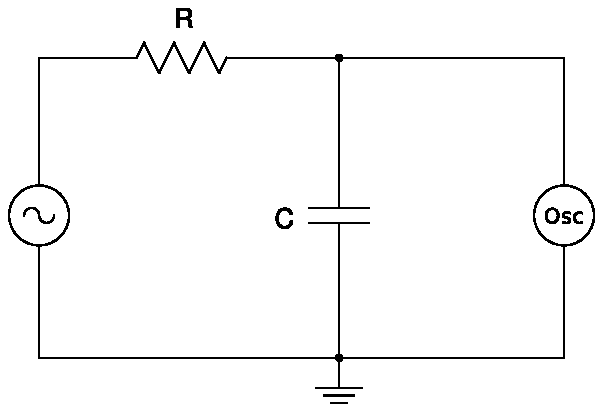
\includegraphics[width=\textwidth]{s_basso.pdf}
                \caption{Passa-basso}
                \label{fig:basso}
        \end{subfigure}%
        ~
        \begin{subfigure}[b]{0.3\textwidth}
                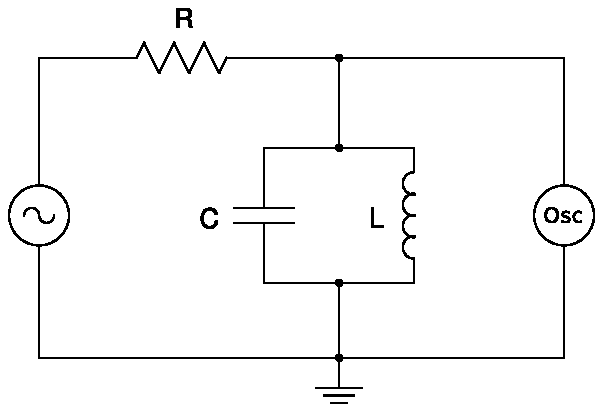
\includegraphics[width=\textwidth]{s_banda.pdf}
                \caption{Passa-banda}
                \label{fig:banda}
        \end{subfigure}
        ~
        \begin{subfigure}[b]{0.3\textwidth}
                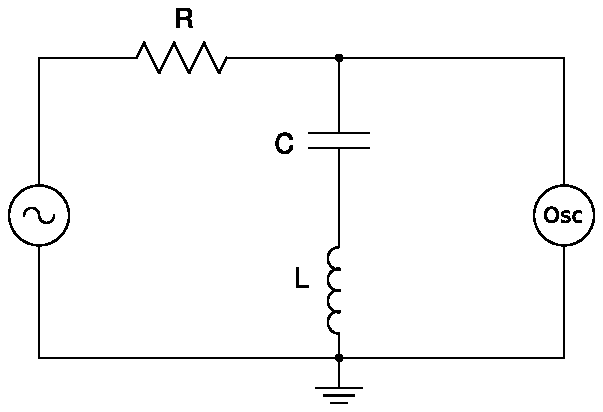
\includegraphics[width=\textwidth]{s_notch.pdf}
                \caption{Reiezione di banda}
                \label{fig:notch}
        \end{subfigure}
\end{figure}
